\documentclass[chap]{thesis}
%indent subsequent lines of captions
\usepackage[labelsep=period,justification=centering]{caption}
%bold caption (needed with caption package to restore boldface.)
\renewcommand{\captionfont}{\bfseries}
%notes to self in color
\usepackage{color}
%Dan: sorts citations like [5, 3, 15] -> [3, 5, 15] !
% -- courtesy of Dan Ibanez
\usepackage{cite}
%Dan: fixes the "numbering starts in the list of figures" problem !
%http://tex.stackexchange.com/questions/36304/ignore-citations-in-captions-in-list-of-figures-when-numbering
%http://ctan.mackichan.com/bibliography/bibtex/contrib/doc/btxFAQ.pdf%
% -- courtesy of Dan Ibanez
\usepackage{notoccite}
%math
\usepackage{amsmath}
\usepackage{amssymb}
%figures - convert eps to pdf files for pdflatex
\usepackage{graphicx}
\usepackage{epstopdf}
%algorithms and pseudo code
\usepackage{algorithm}
\usepackage[noend]{algpseudocode}
%fancy captions for figures
\usepackage{subcaption}
%units for parma tables
\usepackage{siunitx}
%formatting control
\usepackage{placeins}
%import tex and associated files from sub-dirs
\usepackage{import}
%Inferior PDF viewers (Adobe Acrobat lol) create red/green
%blocking around links.
%When using hyperref, but you can't just tell OGE their PDF
%viewers are terrible.
%When submitting your thesis, comment out hyperref
% -- courtesy of Dan Ibanez
\usepackage{hyperref}
%verbatim code listings
\usepackage{listings}
\lstset{language={},basicstyle=\footnotesize\ttfamily}

%The IEEE 2016 Editorial Style Manual does not allow breaks after the ':' char
% so we add it to the default 'url.sty' list of nobreak chars.
\renewcommand*{\UrlNoBreaks}{\do\(\do\[\do\{\do\<\do\:}%

%The IEEE 2016 Editorial Style Manual uses 'Fig.' instead of 'Figure'
\renewcommand{\figurename}{Fig.}

% Attribution of previously published work
% -- courtesy of Justin Lapre
% note, I had to disable the 'alt.interword.spacing' in the IEEE bst file
% https://github.com/SCOREC/scorec-refs/commit/a35abe0e1fe55786c983c65e532636b2beb85a06
% to avoid problems with urls in references
\makeatletter
\def\blfootnote{\xdef\@thefnmark{}\@footnotetext}
\makeatother
\usepackage{bibentry}
\nobibliography*

%formatting parma tables {
\newcolumntype{F}[2]{
  S[table-format=#1.#2,round-integer-to-decimal,round-mode=places,round-precision=#2]%
}
\newcolumntype{E}[3]{
  S[table-format=#1.#2,round-mode=places,round-precision=#2,table-figures-exponent=#3]%
}
%end table formatting }

\begin{document}
%%%%%%%%%%%%%%%%%%%%%%%%%%%%%%%%%%%%%%%%%%%%%%%%%%%%%%%%%%%%%%%%%%%
%                                                                 %
%                            TITLE PAGE                           %
%                            PhD Thesis                           %
%                                                                 %
%%%%%%%%%%%%%%%%%%%%%%%%%%%%%%%%%%%%%%%%%%%%%%%%%%%%%%%%%%%%%%%%%%%
%  This file produces the title page, copyright page (if requested)
%  and the Table of Contents, List of Figures and List of Tables.
%
%  To produce the abstract title page followed by the abstract,
%  see the template file, "abstitle-phd.tex"
%%%%%%%%%%%%%%%%%%%%%%%%%%%%%%%%%%%%%%%%%%%%%%%%%%%%%%%%%%%%%%%%%%%

% Supply information for use on title page:
%
\thesistitle{\bf
Improving Scalability of Parallel Unstructured Mesh-based Adaptive Workflows
}
\author{Cameron Walter Smith}
\degree{Doctor of Philosophy}
\department{Computer Science}
\signaturelines{5}
\thadviser{Mark S. Shephard}
\memberone{Max O. Bloomfield}
\membertwo{Christopher D. Carrothers}
\memberthree{Barbara Cutler}
\memberfour{Onkar Sahni}
\submitdate{April 2017\\(For Graduation May 2017)}
\copyrightyear{2017}

% Print titlepage and other prefatory material:
%
\titlepage
\copyrightpage         % optional
\tableofcontents
\listoftables          % required if there are tables
\listoffigures         % required if there are figures

\specialhead{ACKNOWLEDGMENT}
My seven year mission to seek out new methods for load balancing and building
unstructured mesh workflows was a team effort.
First and foremost, my family and my fiance Alysia provided the much-needed love
and moral support to get through long hours, travel, and times of high stress.
My colleagues Dan Ibanez, Brian Granzow, Seegyoung Seol, Gerrett Diamond, Dan
Zaide, Ben Matthews, Michel Rasquin and many others collectively provided
excellent technical support and devoted many hours to help advance my work.
When my colleagues and I couldn't work out a bug or conceptual issue professors
Ken Jansen, Onkar Sahni, Chris Carrothers, and Scientific Computation Research
Center (SCOREC) research staff member Max Bloomfield provided precious chunks of
their time to help.

Development, testing, and large scale runs were made possible by the staff and
system administrators at the Texas Advanced Computing Center, Argonne National
Laboratory, the SCOREC (Ben Matthews, Tim McMullan and Tim Wickberg), and the
Computational Center for Innovations (Lindsay Todd, Dan Weeks, and Derek Fox)
who kept the software and hardware systems running and up to date.

Thank you to my committee for mentoring me through the Ph.D. program and
reviewing my work.

Last, but not least, thanks to my adviser and boss Mark Shephard for leading my
professional development as a full-time staff member and my research as a
part-time graduate student.
Mark's guidance for navigating complex research topics and, at times, even more
complex institutional bureaucracies, was critical to my success.

\specialhead{ABSTRACT}
High performance parallel adaptive simulations operating on leadership class
systems are constructed from multiple pieces of software developed over many
years.
As increasingly complex systems are deployed new methods must be created to
extract performance and scalability.
This thesis addresses two key scalability limitations for unstructured
mesh-based simulations.

Attaining simulation performance at ever higher concurrency levels requires
increasing the performance of transformations within each procedure, as well as the
transfer of data between procedures.

Controlling the transformations requires distributing the work evenly across the
processors while executing efficient data transfers requires local operations
that avoid shared or contended resources.
This thesis addresses these requirements through multi-criteria load balancing
procedures and in-memory data transfer techniques.

Partition improvement methods defined in this work enable improved application
strong scaling on over one million processors through careful control of the
balancing requirements.
Applied to a computational fluid dynamics simulation running on 524,288
processes with 1.2 billion elements these methods reduce the time of the
dominant computational step by up to 28\% versus the best existing methods.

The scalable data transfer requirement is addressed through an
in-memory functional coupling that avoids the high cost of fileystem access.
The methods developed are applied to adaptive simulations in which
the time required for information exchange is reduced by over an
order of magnitude versus file-based couplings.
Three additional simulations for industrial applications are then provided that
highlight an in-memory coupling and the automation of key simulation processes.

\chapter{INTRODUCTION AND CONTRIBUTIONS}
\label{chp:intro}
\blfootnote{Portions of this chapter have been submitted to:
  C.~W. Smith, B.~Granzow, G.~Diamond, D.~A. Ibanez, O.~Sahni, K.~E. Jansen
  \emph{et~al.}, ``In-memory integration of existing software components for
  parallel adaptive unstructured mesh workflows,'' submitted for publication.}

Unstructured mesh methods, like finite elements~\cite{hughes2012finite} or
finite volumes~\cite{abgrallFiniteVolume2016}, support the
effective analysis of complex physical behaviors modeled by partial differential
equations over general three-dimensional domains.
The most reliable and efficient methods apply adaptive procedures with \textit{a
posteriori} error estimators that indicate where and how the mesh is to be
modified.
Although adaptive meshes can have two to three orders of magnitude fewer
elements than a more uniform mesh for the same level of accuracy, there are many
complex simulations where the meshes required are so large that they can only be
solved on massively parallel systems.

The parallel simulations of interest are defined by a series of procedures which
we refer to as a workflow.
Fig.~\ref{fig:workflow} provides a high-level overview of this sequence.
Starting at the top-left the problem definition is specified on the
computational domain, typically a CAD model.
Next, automated mesh generation procedures driven by the problem definition and
optional mesh controls produce a spatial discretization of the computational
domain, a mesh.
With the mesh, the associated CAD model, and the problem definition, an analysis
is executed until some criterion is met that indicates adaptation is required.
In a workflow using mesh adaptation procedures this criterion is most effective
when it is based on the discretization error~\cite{hughes2012finite}.
Following the analysis, the adaptation procedure is executed to reduce the error
by locally refining and coarsening the mesh~\cite{li20053d,alauzet2006parallel}.
During these mesh modification operations local transfer
procedures~\cite{ibanezthesis} are executed to maintain an accurate
distribution of physical quantities of interest (e.g., the velocity of a fluid
or the displacement of a solid).
Once an adapted mesh has been created, the analysis procedure is executed again.
This solve-adapt cycle is repeated until a stopping criterion is met, such as a
pre-defined number of time/load steps.
After the last cycle completes, post-processing tools are executed to extract
spatial and temporal characteristics of the physical quantities of interest.

\begin{figure} \centering
  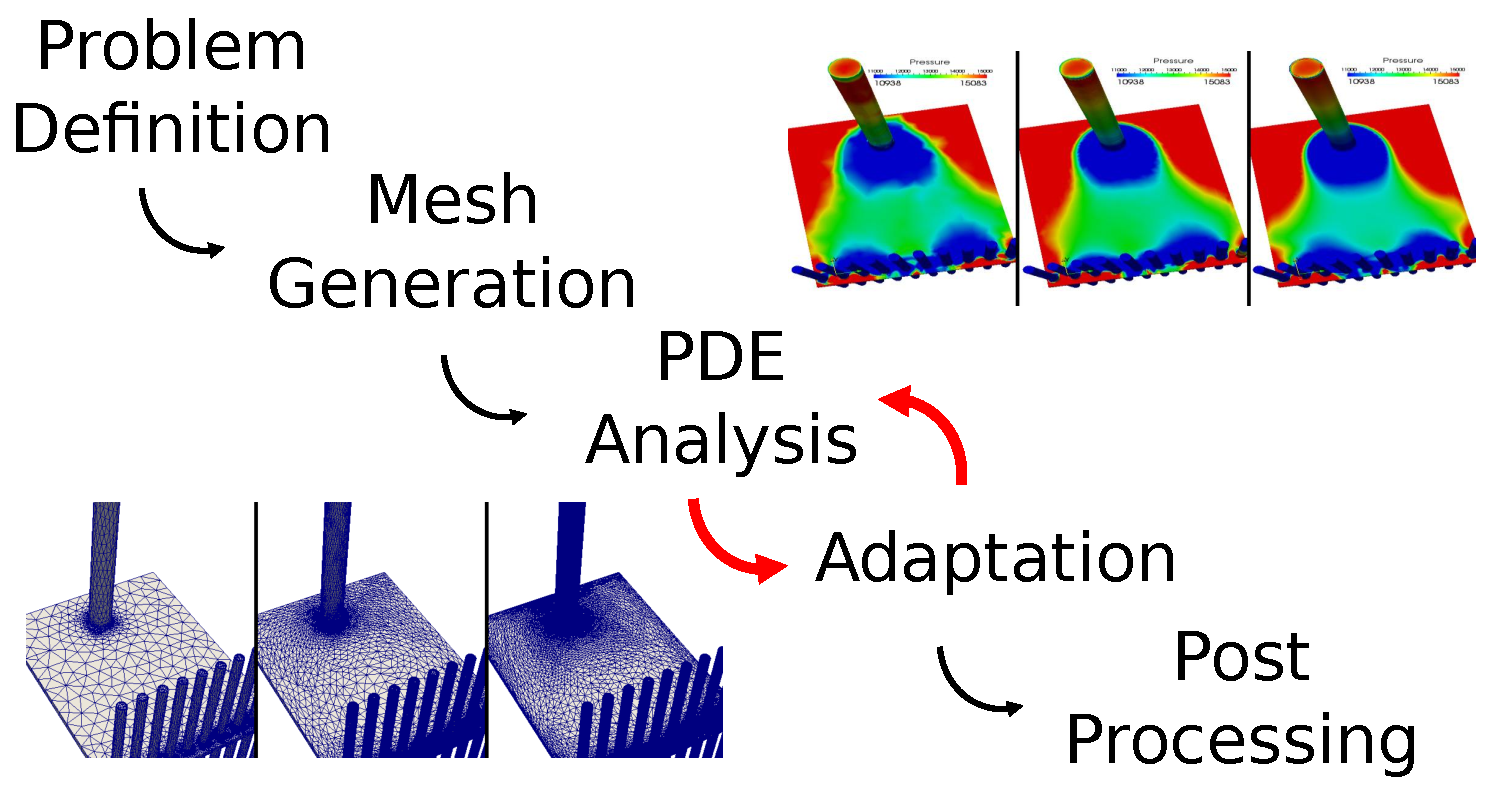
\includegraphics[width=.8\textwidth]{presentation/figs/SimulationBasedEngineeringWorkflow2.eps}
  \caption{
    The series of steps in an adaptive unstructured mesh-based workflow and
    (bottom) a sequence of adapted meshes and (top) the corresponding solution
    fields for an adaptive manifold flow
    simulation~\cite{ovcharenko2013parallel}.
  }
  \label{fig:workflow}
\end{figure}

The time spent running a parallel workflow is dominated by the repeated
execution of PDE analysis and adaptation procedures.
Efficiency of the analysis is maintained by redistributing the mesh after
adaptation procedures have non-uniformly refined and coarsened it.
Given an existing mesh distribution across the processes running on a parallel system,
a partition, dynamic load balancing methods determine which mesh elements should
be moved between processes to reduce the imbalance and communication costs.
For part counts numbering in the tens of thousands, multi-level methods
operating on the dual graph of the mesh are sufficient~\cite{karypis1999parallel}, 
but beyond this concurrency level these methods often fail due to memory usage
that increases significantly with process count~\cite{harlacherMortonSFCvsParmetis2012}.
The goal of \textbf{Par}titioning using \textbf{M}esh \textbf{A}djacencies (ParMA)
is to perform efficient, multi-criteria, dynamic load balancing of
unstructured meshes by directly using the existing mesh adjacency information.
Results will demonstrate the ability of ParMA to dynamically re-balance meshes
for multiple criteria with billions of mesh regions on over one million
processors.
Thus, ParMA addresses a key limitation to workflow scalability by enabling
efficient transformation of data within the computationally dominant analysis
procedures.

Within the solve-adapt cycle are transfers of mesh and field data between
analysis and adaptation procedures (depicted by the pair of bold arrows in
Fig.~\ref{fig:workflow}).
In massively parallel simulations requiring frequent adaptation, the reading and
writing of files between the execution of analysis and adaptation procedures
introduces significant computational overheads.
To avoid shared and contentious parallel filesystems, our in-memory coupling
approaches using data streams and APIs provide scalable and efficient transfers
of data by using node-local memory.
Thus, in-memory transfer approaches address a second key limitation to parallel
workflow scalability.

\section{Contributions}
The work of this thesis develops load balancing and in-memory workflow construction
methods for conformal 2D and 3D unstructured meshes composed of quadrilaterals,
triangles, tetrahedra, prisms, hexahedra, and pyramids.
A conformal mesh is one in which the intersection of two elements is a lower
order mesh entity shared by both (i.e., a face for two regions, an edge for two faces,
and a vertex for two edges).

\subsection{Dynamic Partition Improvement}
ParMA provides dynamic load balancing methods that compliment existing graph and
geometric partitioners to create mesh partitions with billions of elements
on millions of processors that are tailored to the needs of a given application.
Partition improvement results at various per part element counts on over one
million processors are discussed.

\subimport{parmaimprovement/}{parmaContributions}

\subsection{In-memory Component Coupling}
Critical to the construction of parallel workflows is the ability to couple existing
pieces of software.
We define bulk and atomic level couplings implemented using API- and data
stream-based approaches.
These in-memory couplings are applied to a monolithic, mixed C/C++ and FORTRAN,
computational fluid dynamics (CFD) analysis code, a C++, hp-adaptive, finite
element framework for linear accelerator frequency analysis, and a C++
multi-physics framework.
Scaling results up to 16,384 processes are provided for the coupling of the
massively parallel PHASTA CFD analysis code with mesh adaptation, and the memory
overhead for the linear accelerator framework when coupled with mesh adaptation
is studied.

\subsection{Parallel Workflows for Industrial Applications}
In addition to the three in-memory workflows discussed above, we also construct
parallel workflows for three industrial applications.
The first workflow demonstrates an adaptive, multi-phase flow simulation using an
in-memory coupling to a closed-source, serial procedure provided by the
industrial partner.
The second and third workflows focus on reducing the time engineers and analysts
have to spend setting up problems and running jobs by applying automation and
abstraction techniques.

\section{Thesis Organization}
The thesis is organized into the following chapters.
\begin{itemize}
  \item Chapter~\ref{chp:ptnImprovement} details the ParMA load balancing
    software and its support for extreme scale workflows.
  \item Chapter~\ref{chp:workflow} discusses the construction of parallel,
    unstructured mesh-based, in-memory workflows and the components that define
    them.
  \item Chapter~\ref{chp:inmem} describes the in-memory coupling for
    three unstructured mesh-based workflows and examines their performance
    relative to file-based approaches on massively parallel systems.
  \item Chapter~\ref{chp:hpcnyWorkflows} discusses three industrial workflows:
    one using in-memory coupling techniques, and two others using automation
    technologies.
  \item Chapter~\ref{chp:conclusion} summarizes the work and discusses some
    possible future efforts.
\end{itemize}

\section{Terminology and Notation}

\begin{tabular}{l|p{10cm}}
2D,3D              & two- and three-dimensional.\\
petascale,exascale & a computer system capable of executing $10^{15}$
                     and $10^{18}$ floating-point operations
                     per second, respectively.\\
CFD                & computational fluid dynamics.\\
CAE                & computer-aided engineering.\\
CAD                & computer-aided design/drafting.\\
ISV                & independent software vendor; typically a for-profit
                     organization with a closed-source product.\\
I/O                & input and output.\\
API                & application program interface.\\
CPU                & central processing unit; typically a socketed device
                     on the motherboard with multiple, independent, out-of-order
                     processing units.\\
(CPU) core         & a processing unit within a CPU.\\
GPU                & graphical processing unit; typically a bus-attached
                     device with thousands of group-synchronized, simple,
                     in-order processing units.\\
$O(1)$             & an operation that executes in constant time.\\
workflow           & the sequence of steps to set up and execute a
                     simulation.\\
(mesh) part        & a set of mesh elements and their closure assigned
                     to a given process.\\
(mesh) partition   & the set of parts forming a distributed mesh.\\
Ki                 & suffix to denote $2^{10}$. So, for example,
                     16Ki is equal to $16*2^{10} = 16384$.\\
$l.N$              & denotes the $N$th line of an Algorithm or
                     Listing.\\
\texttt{code}      & C/C++/Fortran is written with a fixed-pitch font.
                     For example, the function \texttt{printf(...)} is
                     declared in \texttt{stdio.h}; the ellipsis
                     represent omitted arguments.\\
\end{tabular}

\newpage

The following notation describes the topological entities of geometric models,
meshes, and partitions, the associations between the topological entities, and
the distribution of mesh entities in a partitioned mesh~\cite{ibanez2016pumi}.
\\

\begin{tabular}{l|p{10cm}}
$V$                         & the model, $V$ $\in$ \{$G$, $P$, $M$\}, where
                              $G$ is the geometric model, $P$
                              is the partition model, and $M$
                              is the mesh.
                              \\
$\{V^d\}$                   & the set of dimension $d$ entities in model $V$.\\
$V^d_i$                     & the $i^{th}$ entity of dimension $d$ in model
                              $V$.
                              $d=0$ for vertex, $d=1$ for edge, $d=2$ for
                              face, and $d=3$ for region.\\
\{$M^d_i$\{$M^q$\}\}        & a set of mesh entities of dimension $q$ that
                              are adjacent to $M^d_i$. For instance,
                              \{$M^1_3$\{$M^3$\}\} is a set of mesh regions
                              adjacent to mesh edge $M^1_3$. \\
$M^{d}_i \sqsubset G^{q}_j$ & the geometric classification indicating the
                              unique association of mesh entity $M^{d}_i$
                              with geometric model entity
                              $G^{q}_j$, $d \le q$.\\
$M^{d}_i \sqsubset P^{q}_j$ & the partition classification indicating the
                              unique association of mesh entity $M^{d}_i$
                              with partition model entity
                              $P^{q}_j$, $d \le q$.\\
$w_p(M^d)$                  & the weight of mesh entities $M^d$ on part $p$.\\
$I^d_p$                     & the weighted imbalance of dimension $d$ mesh entities
                              on part $p$;
                              $w_p(M^d_i) / avg(w_{q=0..N-1}(M^d_i))$
                              where $N$ is the total number of parts in the
                              mesh.\\
$I^d$                       & the maximum imbalance of entity dimension $d$;
                              $max(I^d_{p=0..N-1})$.
\end{tabular}

\chapter{IMPROVING UNSTRUCTURED MESH PARTITIONS FOR MULTIPLE CRITERIA USING MESH
ADJACENCIES}
\label{chp:ptnImprovement}
\blfootnote{Portions of this chapter have been submitted to:
C.~W. Smith, M.~Rasquin, D.~Ibanez, K.~E. Jansen, and M.~S. Shephard,
  ``Improving unstructured mesh partitions for multiple criteria using mesh
  adjacencies,'' submitted for publication.
}

\section{Introduction}
Parallel simulation-based engineering workflows using unstructured meshes
require adaptive methods to ensure reliability and
efficiency~\cite{shephard2013bringing}.
Starting with a problem specification on a geometric model~\cite{OBaBea,SheBea},
an effective workflow automatically executes parallel mesh
generation~\cite{tendulkar2011parallel}, analysis, and analysis-based
mesh~\cite{chitale2014anisotropic,Sahn06} and/or
model~\cite{ramm2003error} adaptation.
The analyze-adapt cycle is repeated until a desired level of solution accuracy
is reached.
Between each step in the cycle is an opportunity to improve scalability and
efficiency through dynamic partitioning.

Current dynamic load balancing methods do not effectively reduce imbalances to
the levels needed by applications capable of strong scaling to the full size of
leadership class petascale systems.
This chapter presents a scalable approach that quickly reaches the required
imbalance levels for multiple criteria by pairing Partitioning using Mesh
Adjacencies (ParMA) with current partitioning methods.

\subimport{parmaimprovement/}{parmaSummaryThesis}

\section{Unstructured Mesh Partitioning} \label{sec:partitioning}
\subimport{parmaimprovement/}{parmaBackground}

\section{Dynamic Partitioning Requirements} \label{sec:requirements}
\subimport{parmaimprovement/}{parmaRequirements}

\section{Partitioned Mesh Representation} \label{sec:pumi}
\subimport{parmaimprovement/}{parmaPtnmesh}

\section{Partition Improvement} \label{sec:parma}
\subimport{parmaimprovement/}{parmaPtnimp}

\section{Targeting} \label{sec:targeting}
\subimport{parmaimprovement/}{parmaTargets}

\section{Entity Selection} \label{sec:entSelection}
\subimport{parmaimprovement/}{parmaSelection}

\section{Results} \label{sec:results}
\subimport{parmaimprovement/}{parmaResults}

\section{Summary}
ParMA enables scalable data transformations within components by providing fast,
multi-criteria, dynamic load balancing procedures that execute efficiently on
over one million cores of leadership-class parallel systems.
These procedures rely on part-level (graph distance) and
entity-level (cavity size, surface area) heuristics to define the traversal
order over the part boundary, which elements to select for migration, and the
destination part that should receive the elements.
In addition to the selection heuristics are mechanisms to reject migration
requests if they harm the imbalance of higher priority mesh entities
(cancellation) and to gracefully stop ParMA if beneficial changes can no longer
be made (stagnation avoidance).
The net result of these efforts is a load balancing method that outperforms the
previous versions of the approach (LIIPBMod) in quality and run time, and,
versus a leading graph-based method, improves performance of a massively
parallel CFD code at 512Ki processors by 28\%.

\chapter{CONSTRUCTING PARALLEL ADAPTIVE WORKFLOWS}
\blfootnote{Portions of this chapter previously appeared in:
            \bibentry{shephard2013bringing}}
\blfootnote{Portions of this chapter previously appeared in:
            \bibentry{smithXsede15}}
\label{chp:workflow}
\subimport{workflows/}{wrkflwIntro}
\subimport{workflows/}{wrkflwImpediments}
\subimport{imp/}{impCompInteractions}
\subimport{workflows/}{wrkflwComponents}

\section{Summary}
Parallel workflows for unstructured mesh-based, adaptive simulations are most
effectively constructed from existing software components.
Ideally, these components provide APIs that support bulk (sets of data
over a significant portion of the domain on a given process) or atomic (sets of
data over small sub-domains on a given process) queries and modification
procedures to encapsulated state information.
When the existing software component does not provide these APIs, or provides a
very limited set of them, but supports POSIX file-based interactions, then the
bulk transfer of data into and out of the component is well-supported by
data streams.
Components supporting these bulk and atomic transfers are easily coupled with
other unstructured mesh-based components when their operations are based on a
mesh classified against a geometric and partition model.
PUMI uses this approach for its APIs that query and modify the mesh, its
distribution across processes, and its relation to the geometric model.
PUMI's unstructured mesh components include~\cite{ibanez2016pumi}:
\begin{itemize}
\item PCU - neighborhood-based non-blocking collective communication routines
\item GMI - geometric modeling queries supporting discrete models
  and, optionally, Parasolid, ACIS, and Simmetrix GeomSim models using
  the Simmetrix SimModSuite library
\item MDS - array-based modifiable mesh data structure
\item APF\_MDS - partitioned mesh representation using MDS
\item Field - describes the variation of tensor quantities over the domain
\item ParMA - multi-criteria dynamic load balancing
\item MeshAdapt - parallel, size field driven local refinement and coarsening.
\end{itemize}

\chapter{IN-MEMORY INTEGRATION OF EXISTING SOFTWARE COMPONENTS FOR PARALLEL
ADAPTIVE UNSTRUCTURED MESH WORKFLOWS}
\label{chp:inmem}
\blfootnote{Portions of this chapter have been submitted to:
            \bibentry{smith2017building}}
\subimport{imp/}{impIntro}
This chapter presents the use of in-memory component coupling techniques that
avoid filesystem use for three different unstructured mesh-based, parallel,
adaptive workflows.
These demonstrations highlight the need for in-memory coupling techniques that
are compatible with the design and execution of the analysis software involved.
Key to this compatibility is supporting two interaction modes: bulk and
atomic information transfers.

\section{PHASTA}\label{sec:imp_phasta}
\subimport{imp/}{impPhasta}
\subimport{imp/}{impPhastaDambreak}
\subimport{imp/}{impPhastaPerformance}
\section{Albany Solderball}\label{sec:imp_albany}
\subimport{imp/}{impAlbany}
\subimport{imp/}{impAlbanySolderball}
\section{Omega3P Cavity Frequency Analysis}\label{sec:imp_omega3p}
\subimport{imp/}{impOmega3p}

\section{Summary}
In-memory parallel adaptive workflows for three applications have been
demonstrated using bulk data streams, bulk APIs, and a combination of bulk and
atomic APIs.
The in-memory transfer of data was significantly faster than
file-based transfers for PHASTA and Albany, while the memory overhead for Omega3P
was insignificant.
Key to the three couplings was the use of PUMI's component APIs for queries to, and
modifications of, the mesh, its partitioning, and its associated fields.

\chapter{WORKFLOWS DEVELOPED FOR THE NEW YORK STATE HIGH PERFORMANCE COMPUTING CONSORTIUM}
\label{chp:hpcnyWorkflows}
\blfootnote{Portions of this chapter previously appeared as:
            \bibentry{shephard2013bringing}}
\blfootnote{Portions of this chapter previously appeared as:
            \bibentry{smithXsede15}}

\subimport{applications/}{hpcny}

\section{Summary}
In-memory and semi-automated workflows for three industrial applications were
demonstrated.
For the in-memory PHASTA application the challenge was to work with the
limitations of the industrial partners structural mechanics code while providing
a workflow that efficiently simulated the complex multi-phase flow.
The second and third applications emphasized the definition of workflow
automation to limit the time the analyst or engineer spends setting up problems or
running simulations.

\chapter{CONCLUSIONS AND FUTURE WORK}
\label{chp:conclusion}
\section{Conclusions}

As we move towards the exascale computers being considered \cite{Cross10,Exa10},
it is clear that one of the few effective means to construct parallel adaptive
simulations is by using in-memory interfaces that avoid filesystem interactions.
Of course, the cost of refactoring existing large-scale parallel partial
differential equation solvers to fully interact with the type of structures and
methods used by mesh adaptation components is an extremely expensive and
time-consuming process.
To address these costs, we presented approaches for in-memory integration of
existing solver components with mesh adaptation components, discussed how code
changes can be minimized, and demonstrated the performance advantage within
adaptive simulations.
Demonstrations with the massively parallel computational fluid dynamics, solid
mechanics, and electromagnetics adaptive workflows showed orders of magnitude
performance improvements in I/O procedures using in-memory coupling instead of
files at up to 16Ki processes of the ALCF Theta system.
In addition to efforts on developing in-memory approaches with the PHASTA,
Albany, and Omega3P solvers, efforts are underway to interface other
state-of-the-art solvers including NASA's FUN3D~\cite{anderson1999achieving} and
LLNL's MFEM~\cite{mfem-library}.

Parallel scalability of these workflow components is maintained with
new methods to dynamically balance the computational domain.
These methods work directly on the unstructured mesh alongside traditional graph
and geometric methods to quickly reduce the source of imbalance the
consuming workflow component is sensitive to.
This approach improves the linear algebra work performance of PHASTA
computational fluid dynamics by 28\% over a graph-based partition, and improves
scaling from 0.82 to 1.14, on 512Ki processes of the ALCF Mira system.

As the high performance computing community prepares for near-exascale systems
at the national laboratories, and near-petascale systems become the norm for academia and
advanced industry users, we continue to advance parallel unstructured mesh-based
simulation technologies for efficiently exploiting the massive amount of
computing power on hand and on the horizon.
The challenge is clear; adapt to hardware changes and application needs by
applying new programming and algorithmic approaches while maintaining support
for the existing user base.
We address this challenge by focusing a significant portion of our efforts on
leveraging the wealth of existing components and the thousands of person-hours
invested in them.
In the era of distributed memory message passing between many-core nodes, this
has been a broadly successful approach and is expected to continue well into the
next decade.

\section{Future Work}

\subsection{Partitioning and Load Balancing}

The ParMA load balancing algorithms that worked
directly on unstructured meshes are being generalized to support applications
that use a different mesh distribution (e.g., node partitions), or simply have
information and dependencies between them that can be represented with a graph.
EnGPar~\cite{engpar_github} will implement the ParMA diffusive
algorithms and multi-level graph partitioning procedures using data-parallel
operations on a graph structure using multiple edge-types to represent different
application information dependencies.
Efforts are underway to implement the diffusive algorithms and explore the use
of the Kokkos~\cite{edwards2013kokkos} programming model for
performance portability.

\subsection{In-memory Component Coupling}

Parallel system vendors have started to deploy an additional layer
in the memory hierarchy between the parallel filesystem and main memory (DRAM)
on each node.
The additional layer is implemented by Cray DataWarp devices on the Cori
XC40 system at the National Energy Research Scientific Computing Center.
In the 2018-2019 Aurora system at the Argonne Leadership Computing Facility the
layer will be implemented with Intel SSDs.
By design, we expect transfer tests operating on the new layer to be slower
than data streams and APIs operating out of DRAM or high bandwidth memory.
However, depending on the locality of the SSD or DataWarp devices to compute
nodes, the performance could vary significantly and should be evaluated.

\subsection{Unstructured Mesh-Based Workflows}

Application support using the PHASTA-PUMI and Albany-PUMI
parallel in-memory workflows continues with a fluid structure interaction
problem and an additive manufacturing analysis.
In both cases the coupling approaches developed are reused while specific
aspects of the finite element and mesh adaptivity components are modified.
For PHASTA, developments are focused on implementing the discontinuous
Galerkin method to account for interactions across the solid-gas interface.
In the Albany additive manufacturing workflow the focus is on mesh
adaptation methods to support the evolution of the geometry as layers of
material are deposited.

Ongoing interactions with industrial users are focused on two applications with
evolving geometry.
The first application is simulating flow in a gas filled chamber with a moving
displacer.
Implementation of this workflow requires combining mesh motion to track the
moving geometry and mesh adaptation to maintain element quality.
The second application uses MeshAdapt to support simulation of an underground
reservoir with evolving geometry.

%%%%%%%%%%%%%%%%%%%%%%%%%%%%%%%%%%%%%%%%%%%%%%%%%%%%%%%%%%%%%%%%%%% 
%                                                                 %
%                           BIBLIOGRAPHY                          %
%                                                                 %
%%%%%%%%%%%%%%%%%%%%%%%%%%%%%%%%%%%%%%%%%%%%%%%%%%%%%%%%%%%%%%%%%%% 

\specialhead{REFERENCES}
\bibliographystyle{scorec-refs/IEEEtran_rpi} % specify bibliography style
\begin{singlespace}
\bibliography{scorec-refs/scorec-refs}
\end{singlespace}

% Note that, if you wish, you can use BibTeX to create your bibliography
% from a database. See section 5.6.2 of Memo RPI.110 for information. 
%%% Local Variables: 
%%% mode: latex
%%% TeX-master: t
%%% End: 

\appendix    % This command is used only once!
\addtocontents{toc}{\parindent0pt\vskip12pt APPENDICES} %toc entry, no page #

\chapter{IN-MEMORY EXAMPLE CODE}

\subimport{imp/}{impAppendix}

\end{document}
